\section{Cryptographic Invariant Provenance Graph (CIPG)}
\label{sec:cipg_provenance}

To overcome the static snapshot blind spot and the CA--KDC schema discontinuity identified in Section~\ref{sec:threat_model}, we design the \textbf{Cryptographic Invariant Provenance Graph (CIPG)} (Figure~\ref{fig:neuro_symbolic_pipeline}). CIPG dynamically ingests raw Windows security audit event streams and CA transactional records, maintaining an asynchronous, taint-tracking automaton that bridges disconnected protocol layers.

\subsection{Multi-Source Provenance Ingestion and Entity Resolution}
CIPG processes heterogeneous audit streams across three disjoint operational layers:
\begin{enumerate}
    \item \textbf{Directory Service Audit Events (NTDS):} Monitored via Windows Security Event ID 5136 (\textit{Directory Service Object Modified}). Captures granular LDAP mutations on certificate templates, user objects, and access control lists, recording the modifying principal, target object GUID, modified attribute (e.g., \texttt{nTDSDSOptions}, \texttt{pKIExtendedKeyUsage}, \texttt{msPKI-Certificate-Name-Flag}), and operation type (Value Added / Value Deleted).
    \item \textbf{Certificate Authority Telemetry and CA DB Bridge:} Monitored via Event IDs 4886 (\textit{Certificate Request Received}) and 4887 (\textit{Certificate Issued}). To supply the missing shared certificate identifiers, CIPG queries the local CA transactional database using \texttt{certutil}, requesting the \texttt{RequestID}, \texttt{SerialNumber}, \texttt{SubjectKeyIdentifier}, and \texttt{CertificateHash} fields, or the raw CA RPC interface. This populates a persistent cryptographic tuple:
    \begin{equation}
\fitmath{\begin{gathered}\tau_{\text{crypto}} = \langle \text{Issuer}, \text{RequestID}, \text{SKID},\\  \text{SerialNumber}, \text{Thumbprint}_{\text{SHA1}} \rangle\end{gathered}}
\end{equation}
    \item \textbf{KDC Kerberos Pre-Authentication Events:} Monitored via Event ID 4768 (\textit{Kerberos Authentication Ticket Requested}). Identifies PKINIT authentication requests where \texttt{PreAuthType = 16}, extracting the authenticating client name, domain target, certificate issuer CA, \texttt{CertSerialNumber}, and \texttt{CertThumbprint}.
\end{enumerate}

\begin{figure*}[ht]
\centering
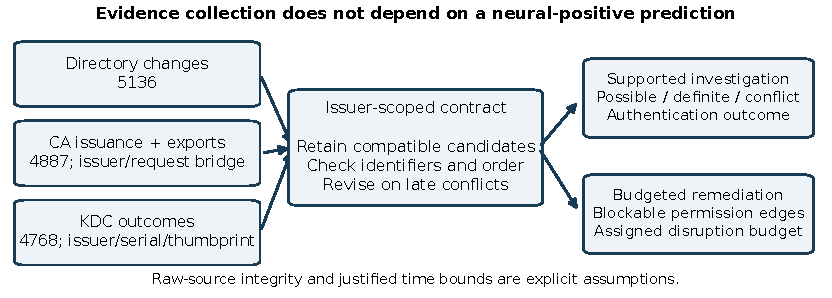
\includegraphics[width=\textwidth]{figures/verified_evidence_pipeline.pdf}
\caption{Certificate-evidence flow through CIPG. Directory changes, CA issuance/export evidence and KDC outcomes support revisable issuer-scoped linkage. Collection is independent of a neural-positive prediction; optional screening cannot discard the long-path positives missed in the evaluated learning study. Remediation retains its separate budget and immutability assumptions.}
\label{fig:neuro_symbolic_pipeline}
\end{figure*}

\subsection{Formal Cryptographic Invariants}
CIPG evaluates incoming event sequences against five formal behavioral and cryptographic invariants:

\begin{definition}[Invariant I: Two-Level Causal Invariant]
Let $e_{\text{mut}} \in \mathcal{E}_{\text{NTDS}}$ be a template ACL or attribute modification executed by principal $u_{\text{actor}}$, and let $e_{\text{req}} \in \mathcal{E}_{\text{CA}}$ be a certificate request submitted for template $t$. Invariant~I is satisfied if:
\begin{equation}
\fitmath{\begin{gathered}t(e_{\text{mut}}) < t(e_{\text{req}}) \\ \land\quad \text{TargetObject}(e_{\text{mut}}) = t \\ \land\quad \text{Requester}(e_{\text{req}}) \in \text{DelegatedPrincipals}(u_{\text{actor}})\end{gathered}}
\end{equation}
\end{definition}

\begin{definition}[Invariant II: Temporal-Order Sequence Invariant]
For any valid certificate lifecycle, the sequence of events must satisfy strict monotone temporal progression:
\begin{equation}
\fitmath{t(e_{\text{mut}}) \le t(e_{\text{req}}) \le t(e_{\text{iss}}) \le t(e_{\text{auth}})}
\end{equation}
This progression refers to effective operations. An audit timestamp inconsistent with it can also arise from clock error, audit delay, or an incorrect event association; it does not alone establish spoofing or replay. When these assumptions cannot be justified, the implementation retains a possible explanation or reports inconsistent evidence.
\end{definition}

\begin{definition}[Invariant III: Principal Identity Discrepancy]
Let $R=\text{Requester}(e_{\text{req}})$ be the Windows security principal submitting the certificate enrollment request, and let $A=\text{TargetIdentity}(e_{\text{auth}})$ be the Kerberos client identity authenticating with the resulting certificate. An identity escalation violation occurs if:
\begin{equation}
\fitmath{R\neq A\quad\land\quad\text{PrivilegeLevel}(A)>\text{PrivilegeLevel}(R)}
\end{equation}
\end{definition}

\begin{definition}[Invariant IV: Rollback Reversal Detection]
Let $e_{\text{mut}}$ be an attribute modification on template $t$ at time $t_1$ adding an insecure flag $\text{attr}_{\text{vuln}}$, and let $e_{\text{roll}}$ be a subsequent modification at $t_3$ deleting $\text{attr}_{\text{vuln}}$. A rollback violation is triggered if:
\begin{equation}
\fitmath{\begin{gathered}\Delta t = t_3 - t_1 \le \tau_{\text{window}} \\ \land\quad \exists e_{\text{iss}} \in \mathcal{E}_{\text{CA}} \text{ s.t. } t_1 \le t(e_{\text{iss}}) \le t_3\end{gathered}}
\end{equation}
where $\tau_{\text{window}}$ is the maximum temporal attack window (configured to 30 minutes in enterprise SOC policies).
\end{definition}

\subsection{Invariant V: Persistent Cryptographic Taint-Flow Automaton}
While Invariants I--IV detect synchronous single-actor attacks, attackers can evade them via two evasive techniques: (i) \textbf{Split-Actor Collusion}, where Actor A mutates the template, Actor B requests the certificate, and Actor A rolls the template back; and (ii) \textbf{Dormant PKINIT Exploitation}, where the attacker delays Kerberos authentication by hours or days until the temporal correlation window $\tau_{\text{window}}$ has expired.

To retain certificate evidence beyond the immediate mutation window, we formalize the \textbf{Persistent Cryptographic Taint-Flow Automaton (Invariant~V)}. Its conclusions depend on captured identity evidence and retained state; it does not guarantee detection over an unbounded history:

\paragraph{Algorithm notation}
Let $\mathcal A_{\mathrm{mut}}$ contain \texttt{nTDSDSOptions}, \texttt{msPKI-Certificate-Name-Flag}, and \texttt{pKIExtendedKeyUsage}. The mutation map $\mathcal M$ stores the object GUID, actor, time and operation. The CA bridge $\mathcal B$ returns the certificate identifiers for an issuer/request pair. A taint entry retains these identifiers, requester, mutation actor and issuance time.

\begin{algorithm}[tbp]
\caption{CIPG certificate-lineage update}
\label{alg:invariant5}
\footnotesize
\begin{algorithmic}[1]
\Require Event stream $\mathcal S$, CA bridge $\mathcal B$, taint table $\mathcal T\gets\emptyset$
\For{each incoming event $e\in\mathcal S$}
 \If{$e.\mathrm{ID}=5136$ and $e.\mathrm{attr}\in\mathcal A_{\mathrm{mut}}$}
  \State Store the mutation in $\mathcal M$
 \ElsIf{$e.\mathrm{ID}=4887$ and its template has an active mutation}
  \State Query $\mathcal B$ using issuer and request ID
  \State Add the resulting taint entry to $\mathcal T$
  \State Retain the certificate as a provisional overlap candidate
 \ElsIf{$e.\mathrm{ID}=4768$ with success and pre-authentication type 15, 16 or 17}
  \State Retain compatible candidates
  \State Reject candidates with a known identifier contradiction
  \If{one strongly identified candidate has justified issuance-before-use order}
   \State Emit the resolved lineage explanation
   \State Distinguish definite from possible mutation overlap
   \State Report mutator, requester and authenticated target
   \State Report authentication-minus-issuance latency
   \State Forward the supported explanation to remediation
  \EndIf
 \EndIf
\EndFor
\end{algorithmic}
\end{algorithm}


Algorithm~\ref{alg:invariant5} illustrates the mutation-taint path. The identity reference also retains unmutated issuances and handles late enrichment and link revision; these broader behaviors are evaluated separately in Section~\ref{sec:evaluation}.

\paragraph{Mathematical Guarantees and Operational Concurrency Realities}
A serial number is scoped to its issuer~\cite{rfc5280}; SKID identifies a public key and can recur across distinct certificates. A thumbprint identifies certificate bytes, while an unauthenticated log field does not itself prove certificate possession or source integrity. The reference implementation requires all shared identity fields to agree and preserves compatible incompletely identified issuances, so missing fields cannot manufacture uniqueness. Late evidence can withdraw a previously resolved link. Retention enables delayed-use analysis only while the necessary observations remain available; no bounded-memory or irreversible-finality guarantee follows.

\paragraph{Bounded-time and source-fault reasoning}
For opening, issuance, and rollback intervals $O,I,R$, definite temporal overlap requires $O^{+}\le I^{-}$ and $I^{+}\le R^{-}$. Otherwise, a feasible overlap remains possible. An exact difference-constraint reference additionally accepts explicitly justified operation-order edges~\cite{dechter1991temporal,amarilli2017order}; contradictory constraints yield an inconsistent-evidence answer. Cross-host record numbers do not supply those edges. This is an application of established temporal reasoning, with certificate-specific evidence requirements.

For a declared optional-export fault budget $k$, let $\mathcal{H}_k$ contain every deletion of at most $k$ CA bridge records. Candidate union over $\mathcal{H}_k$ preserves alternative explanations; a certain link must be resolved to the same issuance in every hypothesis. Abstaining hypotheses are retained, rather than removed to force agreement. If the true issuance is captured, raw issuance/KDC fields and time bounds are correct, and at most $k$ bridge records are faulty, deleting those faulty records leaves a hypothesis containing the true candidate. This is a conditional retention property, not a claim of certain resolution or robustness to compromised raw audit sources. The exhaustive implementation is a correctness reference with combinatorial cost, and source-level compromise can invalidate a record-level budget~\cite{elmagarmid2007duplicate,heinzl2026timestamps}.

The earlier trace-driven synthetic stress stream illustrates two configured trade-offs; its rates do not measure a production deployment:
\begin{enumerate}
    \item \textbf{Background Enrollment Collisions (False Positives):} The configured workload contains 50 maintenance windows with durations in $[10,35]$~s and 2,000 renewals sampled uniformly over the simulated duration. Template selection, rather than the total renewal count, determines the candidate collision rate. Four maintenance windows produce false alarms: $8.00\%$ maintenance-window FPR and $0.0395\%$ overall event FPR, with $92.16\%$ precision at $\Delta_{\text{poll}}=5$~s and $92.31\%$ at 1~s. Section~\ref{sec:evaluation} states the actual sampling scheme; these are synthetic-workload counts, not an enterprise Poisson-rate measurement.
    \item \textbf{CA Database Polling Latency (Simulated False Negatives):} The configured stress stream reports $48/48$ recall at $\Delta_{\text{poll}}=1.0\text{s}$ and $47/48$ at $5.0\text{s}$. These outcomes use the stream's synthetic labels. They are separate from independently checking a successful issuance-to-use chain in captured Windows records; Section~\ref{sec:evaluation} reports that evidence audit.
\end{enumerate}

\subsection{Graph Reduction and Meta-Node Compacting}
Repeated authentication observations can make a provenance graph costly to retain and query. The legacy CIPG implementation groups repeated events into meta-nodes:
\begin{equation}
\fitmath{\mathcal{C}: (v_{\text{event}}^{(1)}, v_{\text{event}}^{(2)}, \dots, v_{\text{event}}^{(m)}) \mapsto \mathcal{V}_{\text{meta}}}
\end{equation}
Whenever repetitive, non-mutating events share identical source principals, destination templates, and access control rights within a sliding window, CIPG collapses them into a single directed meta-edge annotated with frequency counters and temporal bounding intervals $[t_{\min}, t_{\max}]$. As quantified in Section~\ref{sec:evaluation}, this reduces graph storage overhead by \textbf{76.61\%} (compressing 10,182 raw elements to 2,382 compressed elements) while consuming only $6.91$~MB of memory at a sustained ingestion throughput of $13,192.4$~events/second.

\paragraph{Correlated optional sources and self-consistent false order}
Two explicit falsification controls test the boundaries of these guarantees. Six false bridge rows from one exporter exceed a two-record fault budget and produce a wrong certain link. A sufficient six-record reference retains the true candidate with 64 hypotheses; a whole-source deletion reference retains it with two hypotheses under the different assumption of at most one faulty failure domain. It abstains from certainty, and requires an explicitly supplied source partition rather than treating file copies as independent origins. This is a failure-model comparison, not equal-budget accuracy superiority.

A second control supplies true times $o=0$, $c=1$, $i=2$ inside declared bounds $[0,3]$, then fabricates the jointly consistent order $o\le i\le c$. The temporal solver returns definite overlap although the latent history has none. Thus consistency checking cannot authenticate the order channel. The controlled orchestrator is an additional trusted source in our pilot; its truth assumption cannot be replaced by the mere absence of contradictory constraints.
